\section{Box-office influence estimation and prediction}
\label{sec:impact}
An obvious phenomenon is that the box office of movies has significant difference with the year and type.  Similarly, due to the difference of movie types, the original movie ratings can not accurately describe the word of mouth of the movie because of different types. In order to eliminate these effects, we use $BoxScore$ to measure box-office quality of a movie. If there is a movie called $m$ which box office is $boxoffice(m)$ with movie type set $T(m)={T_1,T_2,\ldots,T_k}$ and release year $y(m)$, the $BoxScore$ of $m$ is 
\begin{equation}
BoxScore(m)=\frac{1}{|T|}\sum_{t\in T}\frac{BoxOffice(m)}{\max_{t\in T(n),y(n)=y(m)}BoxOffice(n)}
\end{equation}
and the word of mouth score $WOMScore$ of $m$ is 
\begin{equation}
WOMScore(m)=\frac{1}{|T|}\sum_{t\in T}\frac{WOM(m)-\min_{t\in T(n)}(WOM(n))}{\max_{t\in T(n)}(WOM(n))-\min_{t\in T(n)}(WOM(n))}
\end{equation}
\begin{figure}[!htbp]
\centering
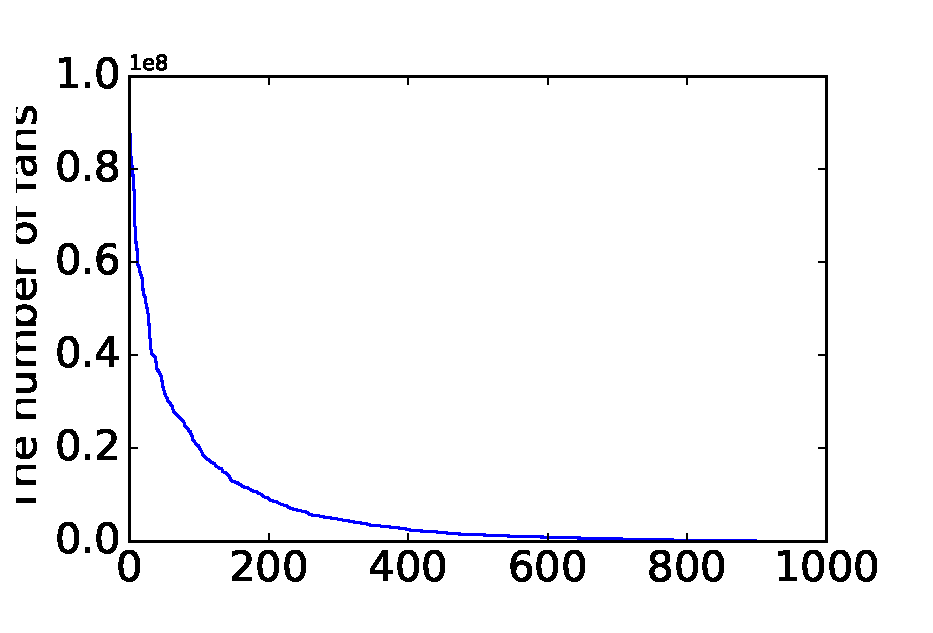
\includegraphics[width=0.8\columnwidth]{distribution.eps}
\caption{Distribution of Fans}
\label{fig:dist}
\end{figure}
\par We provide persona analysis of famous actors and directors which is shown in Figure \ref{fig:screen}. The box office value of a famous director or actor is one of the most important parts of the box office. Famous Cast (directors) are the main performers(directors) over 10 movies or won the film excellent actor(director) award or have more than ten million followers (shown in Figure\ref{fig:dist}) in social networks. Portraying the box office of famous actors or directors in historical movies can help us analyze their value and Volatility.
\par We use $bos,bov,wms,wmv$ to reflect the average box office performance, the box office performance fluctuation, the average word-of-mouth performance and the volatility of word-of-mouth performance so that we can depicte the performance of the historical movie to provide guidance for the selection of the corner. 
\par The goal of this module is to find who is the most bankable person in a movie and to capture the dynamic trends about actors and directors during the period of a movie released. As figure \ref{fig:influ} shows, the box office influences can be made up of three parts: the actors'/directs' own box office appeal, media exposure and feedback from audience. For simplify, we regard actors and directors as creators.
\subsection{Contribution of Cast and Crew}
\begin{figure}[!htbp]
\centering
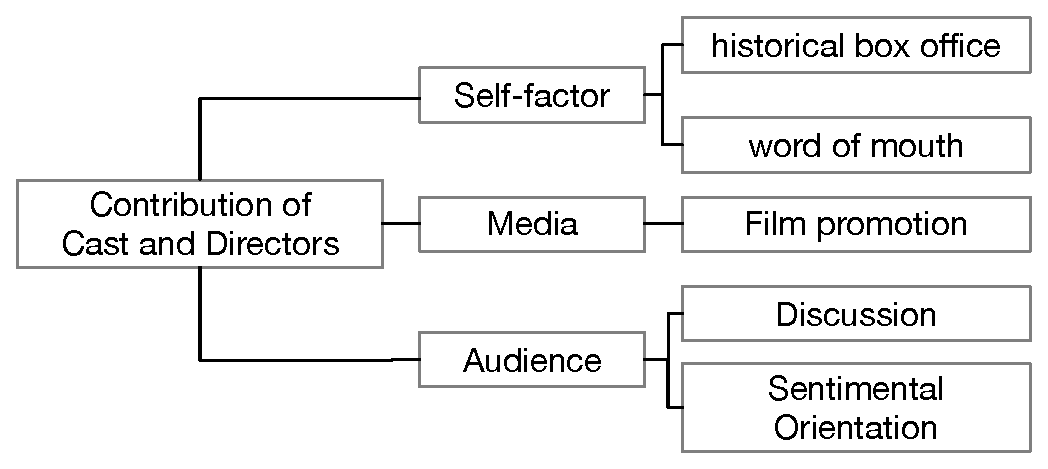
\includegraphics[width=0.8\columnwidth]{contribution.eps}
\caption{Composition of creative influence}
\label{fig:influ}
\end{figure}
\par The creator's own box office appeal. Actor's own box office appeal includes historical box office results and historical word of mouth performance, in which the film's historical movie box office performance can objectively reflect the creative ability of gold absorption, while the historical reputation score can objectively reflect the creative performance by Audience recognition, so this article at the same time using the history of the box office and the history of reputation to measure the creative box office call ability.
\par We define the box office quality $boq$ to measure the box office generated by the creator itself based on the historical film data. 
As for directors, we define 
\begin{equation}
   boq(c)=wms(c)\cdot bos(c)
\end{equation}
Considering different role importance, as for cast, we define 
\begin{equation}
    boq(c) = f(c)\cdot wms(c)\cdot bos(c)
\end{equation}
where $f(c)$ is the influence factor and it depends on the position $k$ that the actor $c$ is. The larger $k$ is , the smaller $f(c)$ gets.
\par Media exposure. The movie's promotional period is always accompanied by a wide range of media coverage, the media's title content reflects the current public focus, if an actor or director appear in the title a lot, you can explain the public familiarity and attention more. We define $meq_j(c)$ as the number of times the creator $c$ referred to by the media in the $j$th week.
\par Feedback from the audience. Liu \cite{liu2006word} mentioned the impact of word-of-mouth on the box office is very large and Craig \cite{craig2015word}added to the equation online buzz variables expressing awareness and purchase intention and examined factors that contributed to higher levels of e-WOM. With the rapid development of the Internet, people can express their emotions on social media at any time. Thanks to the development of social media networks, the promotion of the movie has also gradually increased the proportion of online publicity. At the same time, the content of the discussion of the movie has also formed a considerable amount of data. The movie review often includes the concept of " If you can get the audience's idea of ​​an actor or master from the commentary, you can see whether the source of the audience's emotional inclination toward the movie comes from the influence of the movie's main actor (including the protagonist).We define $aco_j(c)$ as the number of times the creator $c$ referred to by the active comments in the $j$th week.
\par In the short life of the movie, the contribution of the genre to the box office is obviously not constant. With the development of the Internet media, real-time feedback of the movie users on the movie will affect the watching desire of the non-movie users, and the positive contribution Refers to the potential box office or the desire to watch the increase; the negative is the box office to bring the negative image, to dispel the wishes of watching. Therefore, in the film's life, the star effect on the box office's contribution is dynamic, the project will be divided into the life of the movie before the release, the first week of release, the second week of release, the third week of release, released the fourth Friday A period, respectively, to explore the five periods of major box office contributions.
\par We define $DIP_j(c)$ to measure the influence of a famous cast $c$ in $jth$ week
\begin{equation}
DIP_j(c)=w_1\frac{boq(c)}{\sum_{c}boq(c)}+w_2\frac{\sum_{i=0}^{j}mep_j(c)}{\sum_{i=0}^{j}\sum_{c}mep_j(c)}+w_3\frac{\sum_{i=0}^{j}aco_i(c)}{\sum_{i=0}^{j}\sum_{c}aco_i(c)}
\end{equation}
\par Then we can get the DIR (Dynamic Impact Ratio) as $DIR_j(c)=\frac{DIP_j(c)}{\sum_{k\in C}DIP_j(k)}$ to measure the ratio of the box office contribute from creator $c$ to all box box office contribute in $j$th week. Where $w_1$,$w_2$,$w_3$ is three coefficients to embody the importance of creator's own box-office appleal, media exposure and feedback from the audience. The choice of proportion involves expert experience and in practice, we set $w_1=0.1,w_2=0.2,w_3=0.7$.

\subsection{Box-office Predicting}
Movie box office is influenced by many factors, such as investment budget, script, director, actor, post production, producer and producer, media publicity and movie reputation. On the whole, we quantify the factors that affect movie box office from the film itself, the director, the actor and the audience. The opening week due to the lack of effective comments, so just for the release of the film at the box office during the period of life prediction problem, we consider the factors associated with the film at the box office and did not join the historic influence of sentiment analysis, in the opening week after we join in the model of the value of emotional factors.

\label{sec:predict}
\subsection{Premiere week box-office predicting}
\begin{table}[!htb]
  \centering
\begin{tabular}{|c|c|}
\hline
Symbol&Description\\
\hline
$sc$ &The mean $bos$ of famous creators\\
\hline
$gsc$&The mean $wms$ of famous creators\\
\hline
$std$&The variance $bos$ of famous creators\\
\hline
$gstd$&The variance $wms$ of famous creators\\
\hline
$starcounts$& The number of famous creators\\
\hline
$schedule$ & The schedule that the movie came out\\
\hline
$year$ & The year that the movie came out\\
\hline
\end{tabular}
  \caption{Features}
\label{tab:feature}
\end{table}
\par Table \ref{tab:feature} shows the features we used in the task of predicting premiere week box office. As is metioned above, the box office of a movie depends on not only movie factors itself including actors, directors, type, movie propaganda and so on but also influenced by audience reations. In addition, the time the movie released also has a certain impact on the movie box office. In general, predicting premiere week box-office can capture the influences of famous creators(actors and directors) to the movie. We provide Premiere week box-office predicting by using traditional box-office predicting model Support Vector Regression. This Module can help people to asses the influence of stars in the movie.

\subsection{Phased Box-office Predicting}
\begin{figure}[!htbp]
\centering
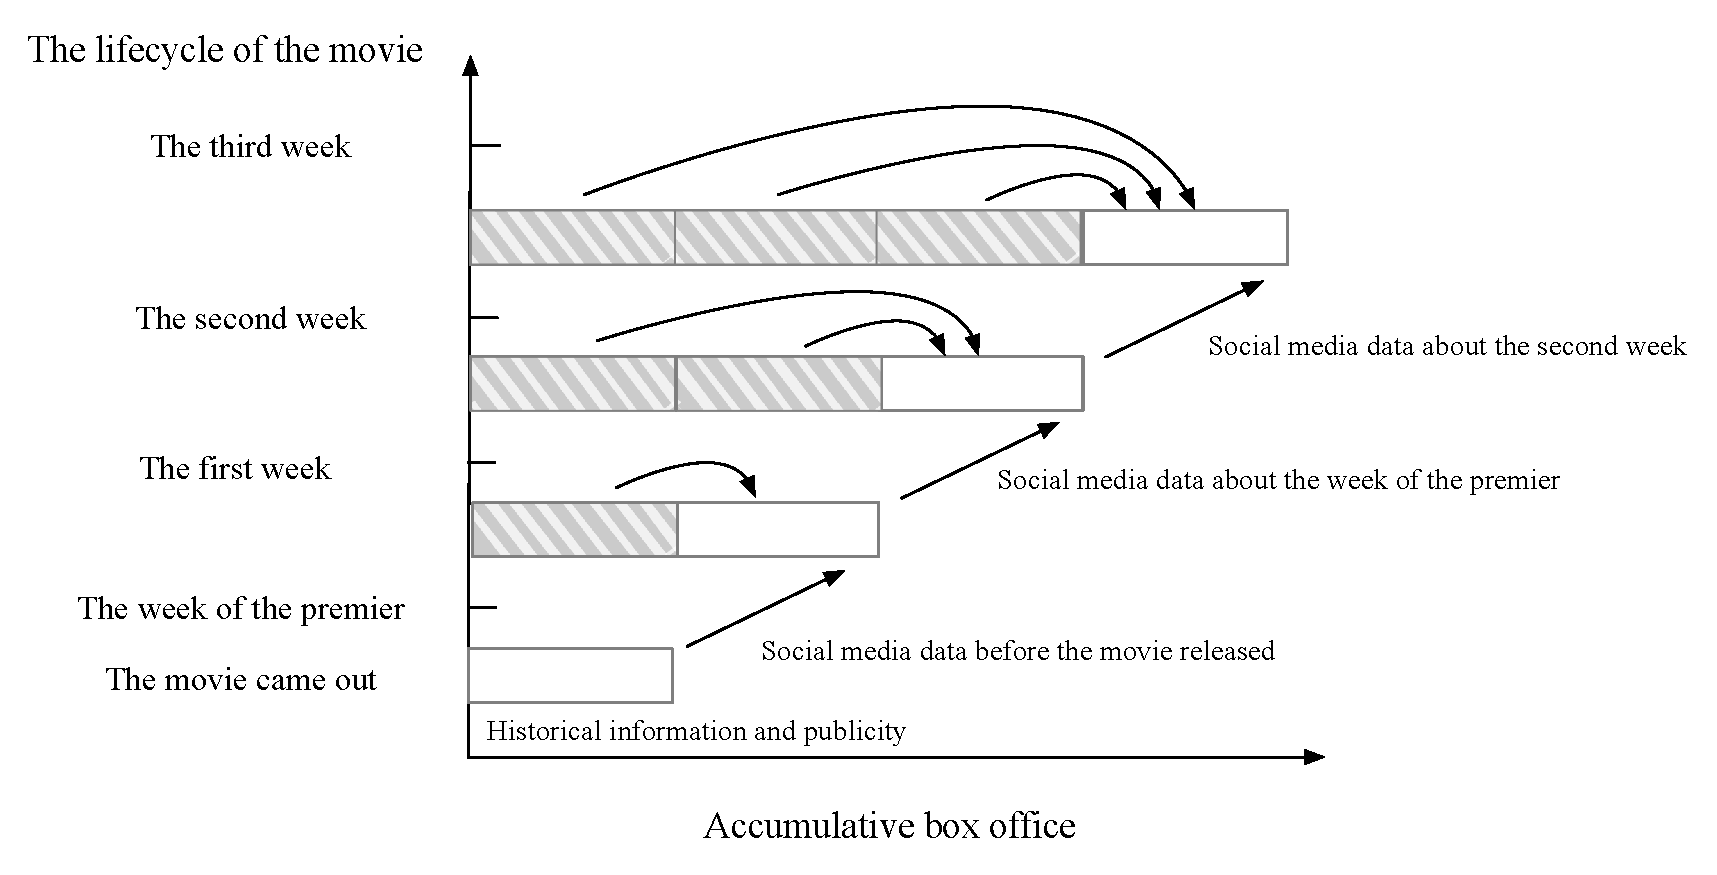
\includegraphics[width=0.8\columnwidth]{boxpredict.eps}
\caption{Multi-stage box office prediction model}
\label{fig:dyna}
\end{figure}
In the past prediction of box office, we usually only forecast the overall box office, but often ignored the movie's influence on movie box office due to the audience's attitude. Such as "wolf 2", the movie box office to be among the world's top 100, because in the release process, because the audience warmly, attracted the audience is not the original film (film series the fans, fans, like the kind of audience) to watch a movie, which leads to the box office continued to rise however, the traditional model is unable to capture this phenomenon. Therefore, as shown in Figure \ref{fig:dyna}, from the pre launch to the 1 months after the release, we set up the box office prediction model with the weekly variation of the weekly release to predict the box office for the first week, the box office for second weeks, the third week box office and the box office at the fourth week.
\par In this section, we add two type features: $weibo_i$, The ratio of creative comments and all comments until the $ith$ week
and $week_i$ The box office in the $ith$ week. With these additional messages obtained from audience and current box office, the results we predict are more similiar to real box office, shown in Table 3.
\begin{table}[!htbp]
\centering
\begin{tabular}{|c|c|c|c|c|c|}
 \hline
    Algorithm\cite{witten2016data} & Metric & First &  Second &  Third &  Forth \\
 \hline
    \multirow{3}{*}{SVR}
    & MSE  & \textbf{0.0939} &  0.2716 & 0.3949 & 0.7445 \\
    & R2score & \textbf{0.6349} & 0.0693& 0.6605 & 0.5734 \\
    & EVC  & \textbf{0.6082} & 0.1977 & 0.7136 & 0.6332 \\
 \hline
     \multirow{3}{*}{RF}
    & MSE  & 0.2683 & 0.3192 & 1.0082 & 0.6839 \\
    & R2score & -1.8019 & -1.0037 & 0.0296 & 0.1461  \\
    & EVC  & 0。4194 & -0.1191 & 0.0253 & 0.4586 \\
 \hline
     \multirow{3}{*}{GBDT}
    & MSE  & 0.6354 &0.5121 &0.7647 & 2.0396   \\
    & R2score & -2.1466 &-0.7831 &0.2974 &0.1664 \\
    & EVC  & 0.2024 &-0.0841&0.6118 &0.0505  \\
 \hline
      \multirow{3}{*}{LR}
    & MSE  &1.0951&0.5105&0.7335&1.3732 \\
    & R2score &-3.5674&-0.7488&0.3694&0.2142  \\
    & EVC  &-3.0608&-0.6947&0.3728&0.3254 \\
 \hline
 	\multirow{3}{*}{LASSO}
    & MSE  &0.7427&\textbf{0.0528}&\textbf{0.0896}&\textbf{0.5025}\\
    & R2score &-2.0977&\textbf{0.8189}&\textbf{0.9229}&\textbf{0.7124}\\
    & EVC  &-0.9281&\textbf{0.9164}&\textbf{0.9758}&\textbf{0.7183}\\
  \hline
\end{tabular}
\caption{Evaluation of Predicting Model}
\label{tab:evalution}
\end{table}